%%%%%%%%%%%%%%%%% DESCRIÇÃO DOS DADOS %%%%%%%%%%%%%%%%%

\chapter{Descrição da base de dados}\label{Sinasc&DNV}


Neste capítulo serão exploradas algumas questões relativas à base de dados utilizada, expondo tópicos sobre seu histórico e estrutura, compreendendo suas limitações e vantagens. Serão detalhados alguns aspectos da variável de interesse, idade do pai, seu período de implementação, assim como será realizada breve análise descritiva do padrão de dados faltantes para a variável por unidade federativa e grande região.   

\section{O Sinasc e a Declaração de Nascido Vivo}

Até a década de 1990 no Brasil, os nascimentos eram registrados no Sistema de Registro Civil. Portanto, se tinha conhecimento apenas dos nascimentos informados em cartório, o que ocasionava um sub-registro \cite{silvestrin2018avaliaccao}. As informações coletadas referiam-se, basicamente, à comprovação legal do evento, sem prover dados importantes para a área de saúde, como as condições da criança ao nascer \cite{szwarcwald2019evaluation}. Em 1989, um grupo assessor foi criado pelo Ministério da Saúde, visando ampliar, reformular e aprimorar o processo de produção e disseminação das Estatísticas Vitais (Gevims), no contexto da informatização dos serviços de saúde e redemocratização do país. O grupo atuou fomentando o debate entre órgãos estaduais responsáveis pela coleta e pela produção de dados da necessidade de implantar um sistema de informação sobre nascidos vivos, o Sinasc. Experiências internacionais e diagnósticos da condição interna dos registros de nascimentos (principalmente da ausência de informações relevantes sobre a saúde dos nascidos vivos) deram base para a necessidade da implementação do sistema e de seu documento base, a Declaração de Nascido Vivo (DNV) \cite{MSsinasc2009}. Nesse contexto, o Sistema de Informações sobre Nascidos Vivos foi implantado pelo Ministério da Saúde em 1990, com a intenção de subsidiar as intervenções relacionadas à saúde da mulher e da criança para todos os níveis do Sistema Único de Saúde (SUS). 

Por meio de diálogo com representantes de todas as unidades da federação foram selecionadas as variáveis para compor a DNV. Alguns dos critérios elencados foram que o documento deveria incluir um número reduzido de variáveis, porém, ao mesmo tempo, contemplar a diversidade regional de serviços de saúde em todo território nacional. Assim, o documento deveria ser adequado para o preenchimento, principalmente, dos profissionais de saúde e, ao mesmo tempo, suprir as necessidades dos gestores de saúde em diferentes níveis de desagregação \cite{MSsinasc2009}. Apesar da imposição legal para a efetivação do fluxo do Sinasc e para a implementação de seu documento base (a DNV) só ocorrer em julho de 1990, impulsionado pela promulgação do Estatuto da Criança e do Adolescente \cite{Lei:8.069:1990}, o sistema foi implementado prontamente pelas Secretarias Estaduais de Saúde \cite{BRMSlegislacao2009}. Ainda assim, devido à vasta extensão territorial brasileira, o desenvolvimento do Sinasc ocorreu de maneira heterogênea no país, fazendo com que os dados do sistema de informação passassem a ser divulgados apenas a partir de 1994 \cite{silvestrin2018avaliaccao}.

Como mencionado, o sistema é alimentado pela DNV, documento obrigatório para a lavratura da Certidão de Nascimento pelos Cartórios do Registro Civil, cujo modelo padrão passa a ser adotado nacionalmente a partir de 1990. A DNV, por definição, notifica o evento vital nascimento, para os nascidos vivos. Quando o produto da gestação não apresenta sinais vitais após a extração, é considerado morto, e apenas seu  óbito é notificado e, em caso de gravidez múltipla, deve ser preenchida uma DNV para cada produto da gestação, ou seja, para cada nascido vivo. Em caso de gestação por substituição (conhecido popularmente por barriga de aluguel) ou de adoção, deve ser considerada a informação da parturiente para preenchimento da DNV, ou seja, a pessoa que gerou e pariu a criança \cite{BRmanualDNV2022}.

Atualmente as unidades notificadoras reconhecidas pelo ministério da saúde\footnote{Art. 13, § 8º, da Portaria nº 116/2009} aptas a receberem formulários de DNV são os estabelecimentos e serviços de saúde (inclusive atendimento e internação domiciliar), profissionais de saúde e parteiras tradicionais vinculadas à unidade de saúde e os cartórios de Registro Civil, que poderão emitir a declaração para nascimentos que tiverem ocorrido a menos de três anos e tenham sido sem assistência de profissionais de saúde ou parteiras \cite{BRmanualDNV2022}. A declaração recebe três vias, a primeira é encaminhada para a Secretaria Municipal de Saúde, a segunda fica com o Cartório de Registro Civil, onde é arquivada no momento da emissão do registro de nascimento, e a última é arquivada no estabelecimento de saúde junto ao prontuário do médico do recém-nascido. 

Segundo o manual mais recente \cite{BRmanualDNV2022}, as DNVs têm como principal fonte as informações prestadas pela(o) parturiente e pelos profissionais de saúde presentes na sala de parto, porém deve-se utilizar também documentos disponíveis, como prontuários, Caderneta da Gestante e anotações pertinentes para auxílio do preenchimento. \citeonline{costa2009avaliaccao} apontam que a DNV pode ser preenchida, nos partos hospitalares, por uma variedade de profissionais de saúde. Entre obstetras, pediatras, enfermeiros-assistentes da sala de parto, estagiários, auxiliares de enfermagem, funcionários administrativos, entre outros, muitos dos quais não estarão necessariamente qualificados para a função. 

Muitos fatores podem afetar a qualidade das informações contidas no Sinasc \cite{bonilha2018cobertura}. Desde problemas no treinamento dos profissionais responsáveis pelo preenchimento que podem afetar a qualidade dos dados (problemas de incompletude e validade dos registros), da disposição das pessoas e instituições em participar e conduzir o sistema, ou questões relacionadas ao funcionamento do Sinasc, nível de cobertura, rapidez na inclusão do nascimento.

A avaliação de cobertura do Sinasc, diz respeito ao quanto dos nascimentos que ocorrem no país tem sido realmente registrados no sistema, e pode ser avaliada utilizando a razão entre Nascidos Vivos Informados e Estimados (via estatísticas oficiais produzidas no Censo Demográfico, Contagem Intercensitária, Pesquisa Nacional por Amostra de Domicílios, estimativas e projeções demográficas), onde valores abaixo de 100 indicam sub-registro do Sinasc \cite{rede2002indicadores}. Alguns autores demonstram como esse aspecto foi melhorando através do tempo \cite{gabriel2014evaluation, bonilha2018coverage}. Estima-se que na década de 1980, antes da implementação do Sinasc, o sub-registro do evento era da ordem de 22,6\% no país \cite{IBGEVitais1980}. Em 1994, ano em que passam a ser divulgados os dados do Sinasc, a região Norte e Nordeste apresentaram os piores valores para a Razão de nascidos vivos informados e estimados, de 65,5\% e 54,9\%, respectivamente \cite{rede2002indicadores}. Porém, o sistema foi se consolidando, em 2004 o Brasil apresentava uma cobertura de 89,4\%. Mais recentemente tem sido testada uma metodologia chamada “Técnica de Captura-Recaptura”\footnote{\href{https://biblioteca.ibge.gov.br/visualizacao/livros/liv101927.pdf#page=11.45}{IBGE. Estudo Complementar à Aplicação da Técnica de Captura-Recaptura Estimativas desagregadas dos totais de nascidos vivos e óbitos 2016 - 2019. Rio de Janeiro, 2022.}}, onde é feito o pareamento dos nascimentos registrados no Sinasc e aqueles contabilizados nas Estatísticas do Registro Civil, com o intuito de avaliar a cobertura do sistema. Ainda que seja uma estatística experimental\footnote{i.e. que estão sob avaliação porque ainda não atingiram um grau completo de maturidade em termos de harmonização, cobertura ou metodologia.}, é possível observar dos nascidos vivos no Brasil no ano de 2022, a proporção de subnotificação foi de 0,45\%, para partos realizados em hospitais, 1,01\% para partos realizados em outro estabelecimento de saúde sem internação, 4,07\% em partos domiciliares e 4,30\% na categoria  “outros” \footnote{\href{https://www.ibge.gov.br/estatisticas/sociais/populacao/26176-estimativa-do-sub-registro.html?edicao=32265\&t=resultados}{IBGE - Sistema de Estatísticas Vitais: Tabela 1.2}}. Demonstrando que, mesmo em partos realizados fora do ambiente hospitalar, o sistema parece estar próximo de uma cobertura completa.

A acurácia diz respeito à confiabilidade ou validade dos dados registrados. Segundo \citeonline{MSsinasc2009}, à data do documento, não existiam rotinas previstas no sistema para a avaliação da acurácia das informações. No entanto, autores brasileiros têm se debruçado sobre o tema, comparando principalmente as informações inseridas no Sinasc com dados do prontuário médico ou por meio de entrevistas com as mães. \citeonline{almeida2006validade}, por exemplo, mostraram problemas de acurácia nas informações sobre as condições socioeconômicas (grau de instrução/escolaridade, estado civil) das mães.

Outro aspecto fundamental para a qualidade do Sinasc é avaliar se os documentos estão sendo preenchidos de maneira adequada, saber quantos dos registros existentes no sistema apresentam informação
ou, então, saber a proporção de registros com informação em branco ou ignorada, i.e., a completude. Altos níveis de incompletude podem indicar a necessidade de treinamento para preenchimento de determinadas variáveis, que podem estar gerando dúvidas ou mesmo que não estão sendo consideradas relevantes pelos responsáveis pelo preenchimento da DNV.  

\citeonline{completude_sinasc} avaliaram, a partir dos dados tabulados do Sinasc\footnote{Extraídos a partir do tabulador de dados do Sinasc: \href{https://datasus.saude.gov.br/informacoes-de-saude-tabnet/}{Tabnet.}} a completude de algumas variáveis ao longo do tempo. Demonstraram que, de maneira geral, as variáveis disponibilizadas no tabulador demonstraram uma tendência de queda para os campos marcados como “ignorado”. Avaliando a completude por meio de uma métrica composta das médias das proporções de grupos de variáveis, onde se calculou a média das médias dos grupos para fazer uma comparação entre as Unidades Federativas (UFs). Identificaram que, nos anos em que algumas variáveis foram implementadas, como Consultas pré-natal e raça/cor, houve picos de não preenchimento. A região Norte e Nordeste apresentaram maiores proporções de campos ignorados no início do período analisado (1994), porém melhorando a cobertura a medida do tempo. 

\begin{grafico}
    \centering
     \caption{Métrica de qualidade do preenchimento dos dados de nascimentos por UF e ano}
    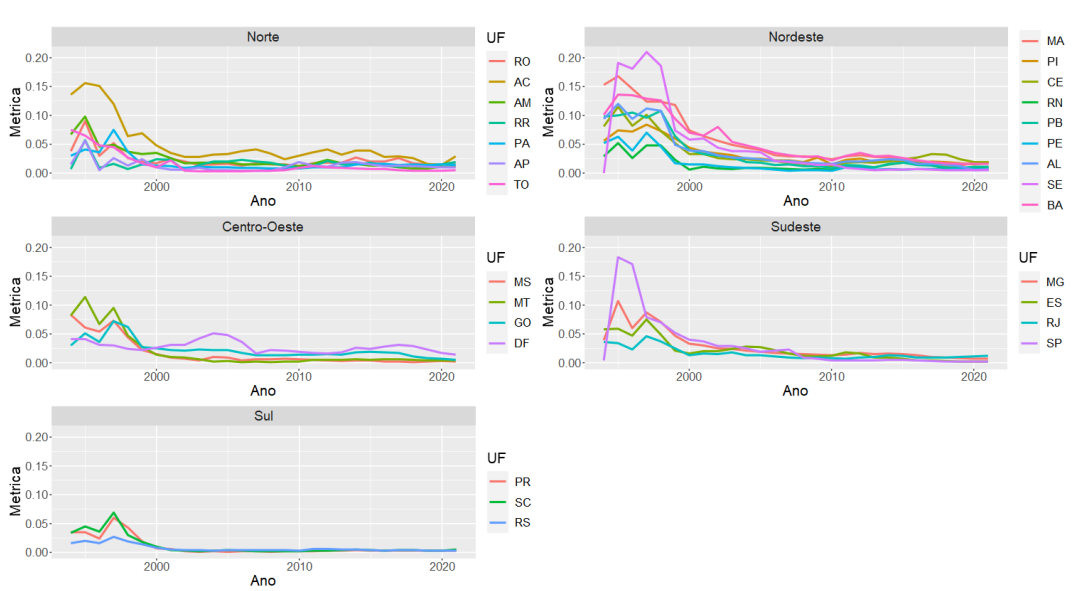
\includegraphics[width=6in]{imagens/o-que-se-tem.PNG}
     \legend{\footnotesize Legenda: Valor zero representa preenchimento de todos os campos. Quanto mais distante de zero, maior o uso das categorias “ignorado” e afins.}
    \fonte{\citeonline{completude_sinasc}}
\end{grafico}


Apesar de \citeonline{completude_sinasc} identificarem uma melhora no preenchimento das variáveis do Sinasc ao longo do tempo, sua análise não contempla a variável para idade do pai ou responsável, que não é disponibilizada através do tabulador Tabnet, apenas disponível através dos microdados. Embora a completude do sistema, de maneira geral, apresente melhorias, parece haver diferenças regionais e estaduais quanto à observação do campo idade do pai ou responsável, como veremos na próxima seção. Uma hipótese é de que possíveis diferenças na postura das Secretarias Municipais de Saúde (SMS) em relação ao preenchimento da variável podem ter afetado a relevância dada ao quesito.

A versão da DNV em uso foi atualizada em 2021 e é composta por 52 variáveis, distribuídas em oito blocos: I - IDENTIFICAÇÃO DO RECÉM-NASCIDO (seis variáveis: data, hora, sexo, raça/cor do recém-nascido, peso ao nascer, Índice de Apgar, detectada alguma anomalia congênita), II - LOCAL DA OCORRÊNCIA (sete variáveis: local da ocorrência, estabelecimento, endereço da ocorrência, CEP, bairro/distrito, município de ocorrência, UF), III - PARTURIENTE (14 variáveis: nome, cartão SUS, escolaridade (última série concluída), ocupação habitual, data nascimento, idade, naturalidade, situação conjugal, raça/cor, residência, logradouro, CEP, bairro/distrito, município, UF), IV -RESPONSÁVEL LEGAL (duas variáveis: nome, idade), V - GESTAÇÃO E PARTO (11 variáveis: histórico gestacional, data da última menstruação (DUM), número de semanas de gestação, número de consultas de pré-natal, 34 Mês de gestação em que iniciou o pré-natal, tipo de gravidez, apresentação\footenote{Com relação ao recém nascido. As opções são: 1 – Cefálica; 2 – Pélvica ou Podálica; 3 – Transversa 9 – Ignorado.}, o trabalho de parto foi induzido?, tipo de parto, cesárea ocorreu antes do trabalho de parto iniciar, nascimento assistido por), VI - ANOMALIA CONGÊNITA (uma variável de campo aberto para descrever todas as anomalias congênitas observadas no recém-nascido. ), VII - PREENCHIMENTO (seis variáveis: data do preenchimento, nome do responsável pelo preenchimento, função, tipo documento, número do documento, órgão emissor), VIII - CARTÓRIO (cinco variáveis de preenchimento exclusivo do Oficial do Registro Civil (cartórios): cartório, registro, data, município, UF)\cite{BRmanualDNV2022}.

A disponibilização do banco de dados consolidado ocorre a cada dois anos, devido aos processos de aprimoramento e qualificação dos dados de natalidade. Esses processos são realizados em três etapas junto aos estados e municípios onde há procedimentos de crítica dos dados, mediante checagem de inconsistências e possíveis duplicidades\footnote{\href{https://svs.aids.gov.br/daent/centrais-de-conteudos/dados-abertos/sinasc/}{Sistema de Informações sobre Nascidos Vivos (SINASC) - Nota Informativa.}}. Por esse motivo, nossa análise se limitará ao ano de 2022.

%

\section{Idade do pai ou responsável ao nascimento}\label{var_interesse}

Nossa variável de interesse, relativa à idade do pai, apresenta pouca documentação acerca de sua implementação e manutenção no Sinasc. A DNV passou por alguns processos de atualização. \citeonline{jorge2007quality} afirmam que no primeiro modelo de DNV estavam presentes campos para registros das seguintes informações: cartório de registro e o local de ocorrência do nascimento, informações sobre o recém-nascido (data do nascimento, sexo, peso ao nascer, índice de Apgar) e sobre a gravidez (duração da gestação, tipo de gravidez e tipo de parto), características da mãe do nascido vivo (nome, idade, grau de instrução, município de residência e filhos tidos) e nome do pai. Porém, em janeiro de 1996, já passa a circular um novo modelo de DNV no país, no qual o campo para registro do nome do pai foi retirado \cite{jorge2007quality}.

\citeonline{mello1993avaliaccao} já apontavam (quando o sistema de informação sobre nascimentos era ainda operado pelo Instituto Brasileiro de Geografia e Estatística, com base nas informações do Registro Civil) sobre comportamento atípico para a variável nome do pai, em relação às demais onde, segundo eles, “a ausência de informação, neste caso, não implica, necessariamente, falha de preenchimento, podendo, também, retratar o desejo de não identificar o pai.” \cite[p.21]{mello1993avaliaccao}. Relataram, ainda, que no estudo que realizam em cinco municípios de São Paulo, um dos municípios não possuia registro para a informação porque o único hospital da cidade\footnote{Município de Pariquera-Açu.}, à época, decidiu deliberadamente omitir o dado. Concluíram que a informação relativa ao nome do pai estava sendo pouco valorizada pelos estabelecimentos de saúde. Em trecho que exprimem sua opinião, os autores afirmam: “Essa atitude vem ao encontro de opinião dos autores que julgam ser o nome do pai uma informação de caráter jurídico e não médico, epidemiológico, ou de saúde pública e, portanto, dispensável em um documento dessa natureza.”\cite[p.21]{mello1993avaliaccao}.

Não foi possível verificar porque o campo (nome do pai) foi retirado em 1996, já no âmbito do Sinasc. Somente através do dicionário de variáveis disponível no site da Secretaria de Vigilância em Saúde e Ambiente \footnote{Fonte: \href{https://svs.aids.gov.br/daent/cgiae/sinasc/documentacao/dicionario_de_dados_SINASC_tabela_DN.pdf}{Dicionário de dados da tabela DN.}} foi possível identificar que as variáveis que registram informações sobre a paternidade do nascido vivo (a saber, nome e idade do pai) fazem parte de um conjunto de novos campos criados em 2009. 

A mudança da DNV em que é introduzida, aparentemente, pela primeira vez, o registro da idade do pai ao nascimento, foi discutida e aprovada no Comitê Técnico Assessor do SIM (Sistema de informação sobre Mortalidade) e Sinasc no período de 2007 a 2009 \cite{BRConsolidacaoSINASC2011}. O processo de implementação se deu de forma gradual, após realização de teste piloto, o novo formulário foi ajustado e impresso em 2010. O CTA decidiu por uma estratégia de não substituir abruptamente a DNV antiga pela nova versão, fazendo com que o modelo antigo e o novo circulassem simultaneamente.

Apesar da orientação de que, a partir de janeiro de 2011, fosse utilizado preferencialmente os formulários novos, naquele ano ainda houve uma proporção expressiva dos nascimentos sendo registrados no modelo antigo da DNV. Segundo relatório da Coordenação Geral de Informações e Análise Epidemiológica \cite{BRConsolidacaoSINASC2011}, a base de dados do Sinasc de 2011 é constituída de 58\% de formulários novos (com informação para idade do pai), e 42\% de formulários antigos. Por região, a participação do formulário novo variou, sendo maior no Nordeste (88\%), e menor no Sudeste (35\%). O Centro-Oeste teve, proporcionalmente, a segunda maior utilização de formulário novos (76\%), seguido pelo Norte (68\%), e pelo Sul (39\%). Devido aos campos com informações sobre a paternidade serem coletados somente a partir do novo modelo adotado em 2009, a análise terá início em 2012.

Em sua última atualização, o 8º modelo da DNV distribuído a partir de agosto de 2021, os campos para registro de informações paternas foram modificados, para se adequar a novos modelos de parentalidade e arranjos familiares\footnote{Fonte: NOTA TÉCNICA Nº 195/2021-CGIAE/DASNT/SVS/MS. Disponível em: https://dive.sc.gov.br/phocadownload/SINASC/Legisla\%C3\%A7\%C3\%A3o/NTF-n195-2021.pdf}.
O “bloco IV - Pai”, contendo o nome e idade do pai, passa a ser “Bloco IV– Responsável legal”, onde deve ser registrado o nome do(s) responsável(eis) legal(ais)\footnote{É possível registrar, inclusive, dois responsáveis legais, nesse caso, fica registrada a idade do  primeiro responsável legal inscrito.} \cite{BRmanualDNV2022}. Os campos para registro das informações paternas, desde sua implementação 2009-2010, não são de preenchimento obrigatório e não é necessário, nem suficiente, para o reconhecimento da paternidade. Ou seja, ter o nome do pai registrado na DNV não dá legitimidade legal à paternidade do nascido vivo, esse procedimento é somente realizado em cartório \cite{BRmanualDNV2011}. A não utilização dos termos “pai” e “mãe” ocorre para que seja contemplada a filiação, independentemente da identidade de gênero, como nos casos de reprodução assistida, casais transgêneros, união homoafetiva e outras situações similares. Nos campos para “Responsável legal” não têm, necessariamente, a idade do genitor do nascido vivo registrada. Porém, admite-se que o registro de nascimentos havidos por reprodução assistida ou de gestação por substituição ainda ocorram em proporção tal que não devem alterar as estimativas.

Fazendo uma avaliação da completude do preenchimento para a variável idade do pai ou responsável no Sinasc, podemos avaliar que 2012 foi o ano com menor proporção de registros ignorados. No decorrer dos anos, a completude da variável apresenta piora, chegando a mais de 60\% de dado faltante de 2018 em diante (gráfico \ref{graf:FaltanteBrasil})\footnote{Os gráficos apresentados nessa seção serão alterados para contemplar os anos de 2021 e 2022.}. Tal comportamento pode decorrer da falta de valorização destinada à variável, como ilustrado pela perspectiva de \citeonline{mello1993avaliaccao}, da percepção dessa informação como algo não associado à saúde pública ou sem valor jurídico (para a afirmação da paternidade) e, portanto, vista como não valiosa para o contexto do documento. 

\begin{grafico}
    \centering
    \caption{Percentual de dados faltantes para a idade do pai ou responsável - Brasil - 2012-2020}
    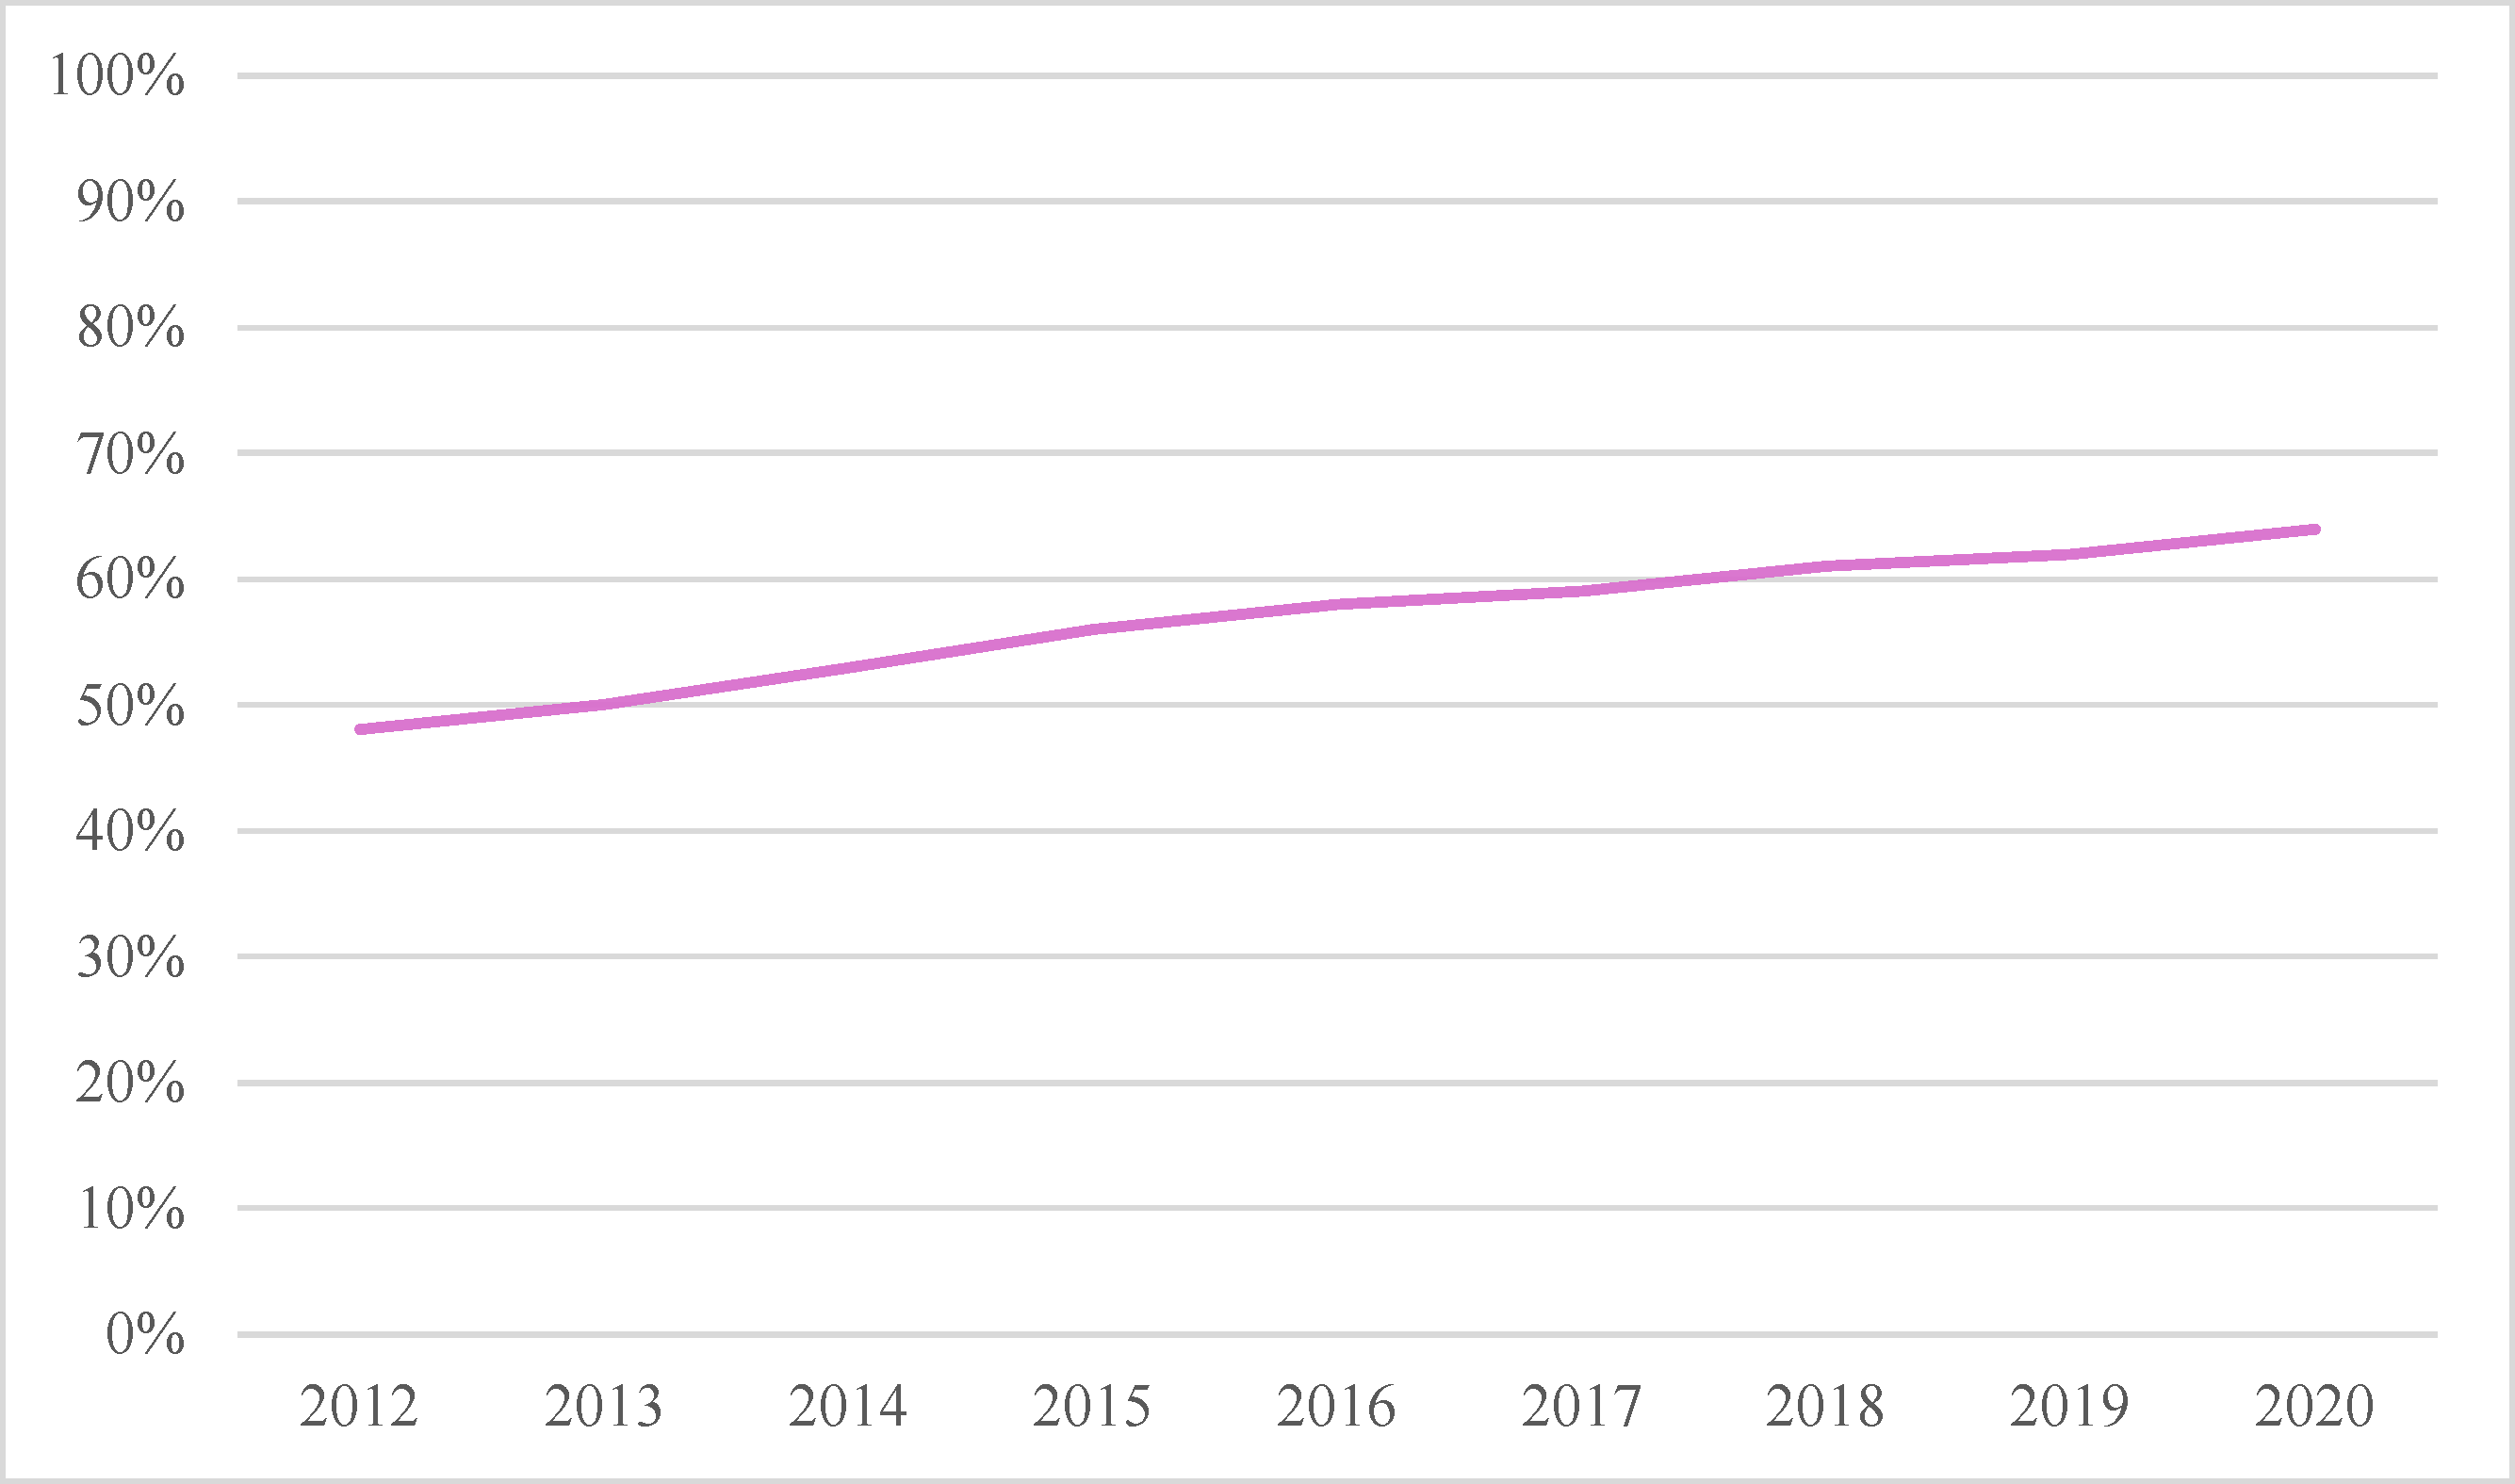
\includegraphics[width=5.0in]{imagens/Proporção de dados faltantes para idade do pai 2010-2020 nível Brasil.pdf}
    \fonte{Datasus - Sinasc}
    \label{graf:FaltanteBrasil}
\end{grafico}

A distribuição dos valores faltantes não acontece de maneira homogênea entre as regiões e UFs. Observando os gráficos \ref{graf:sudeste} ao \ref{graf:nordeste} vemos comportamentos diferentes. A região Sudeste apresenta percentuais semelhantes de valores faltantes entre as UFs, com valores concentrados entre 30\% e 40\% no início do período e entre 50\% e 60\% em 2020.

\begin{grafico}
    \centering  
    \caption{Percentual de dados faltantes para a idade do pai ou responsável - Região Sudeste - 2012-2020}
    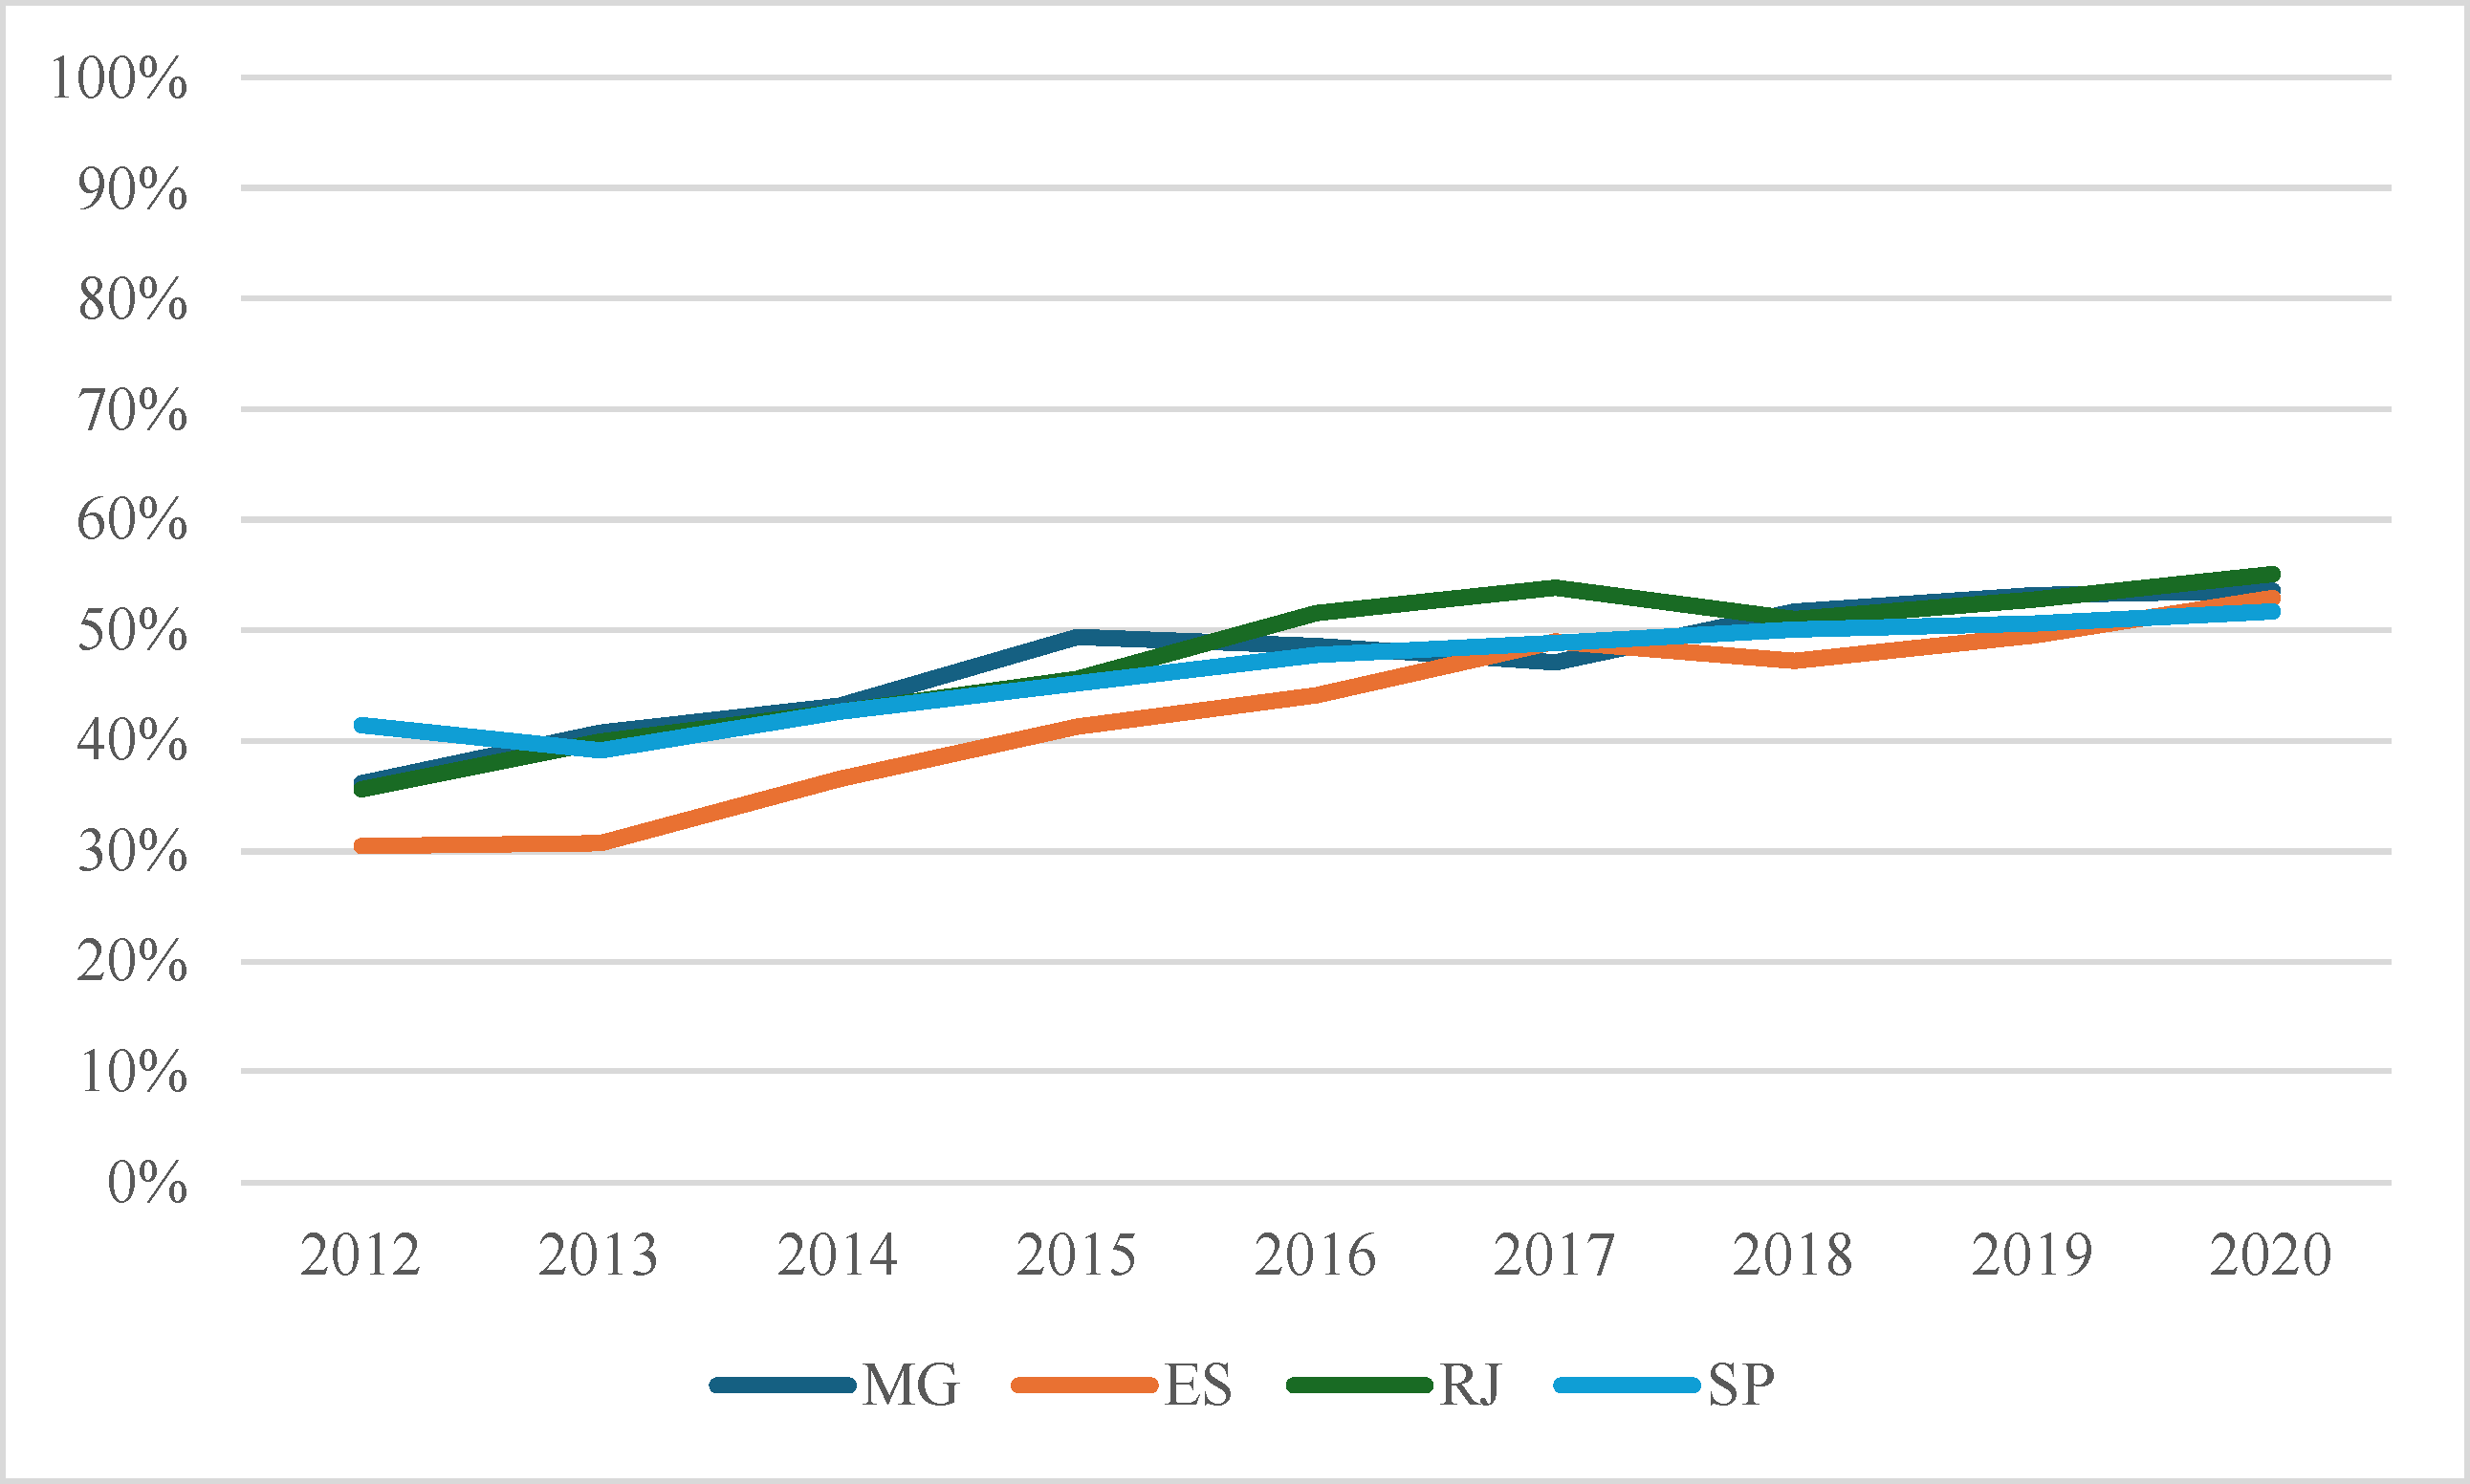
\includegraphics[width=5.0in]{imagens/faltantes-sudeste.pdf}
    \fonte{Datasus - Sinasc}
    \label{graf:sudeste}
\end{grafico}

Já os valores para o gráfico \ref{graf:sul} são mais discrepantes entre os estados, com Santa Catarina apresentando 45\% de dado faltante em 2012, enquanto Paraná o valor encontrado foi de 13\% para o mesmo ano. O Paraná foi a UF que apresentou as menores proporções de dados faltantes no período. Observa-se, porém, que o padrão de crescimento da não observação da idade do pai também ocorre no estado, alcançando o mesmo nível de dado faltante que o Rio Grande do Sul em 2020, em 33\%.

\begin{grafico}
    \centering  
    \caption{Percentual de dados faltantes para a idade do pai ou responsável - Região Sul - 2012-2020}
        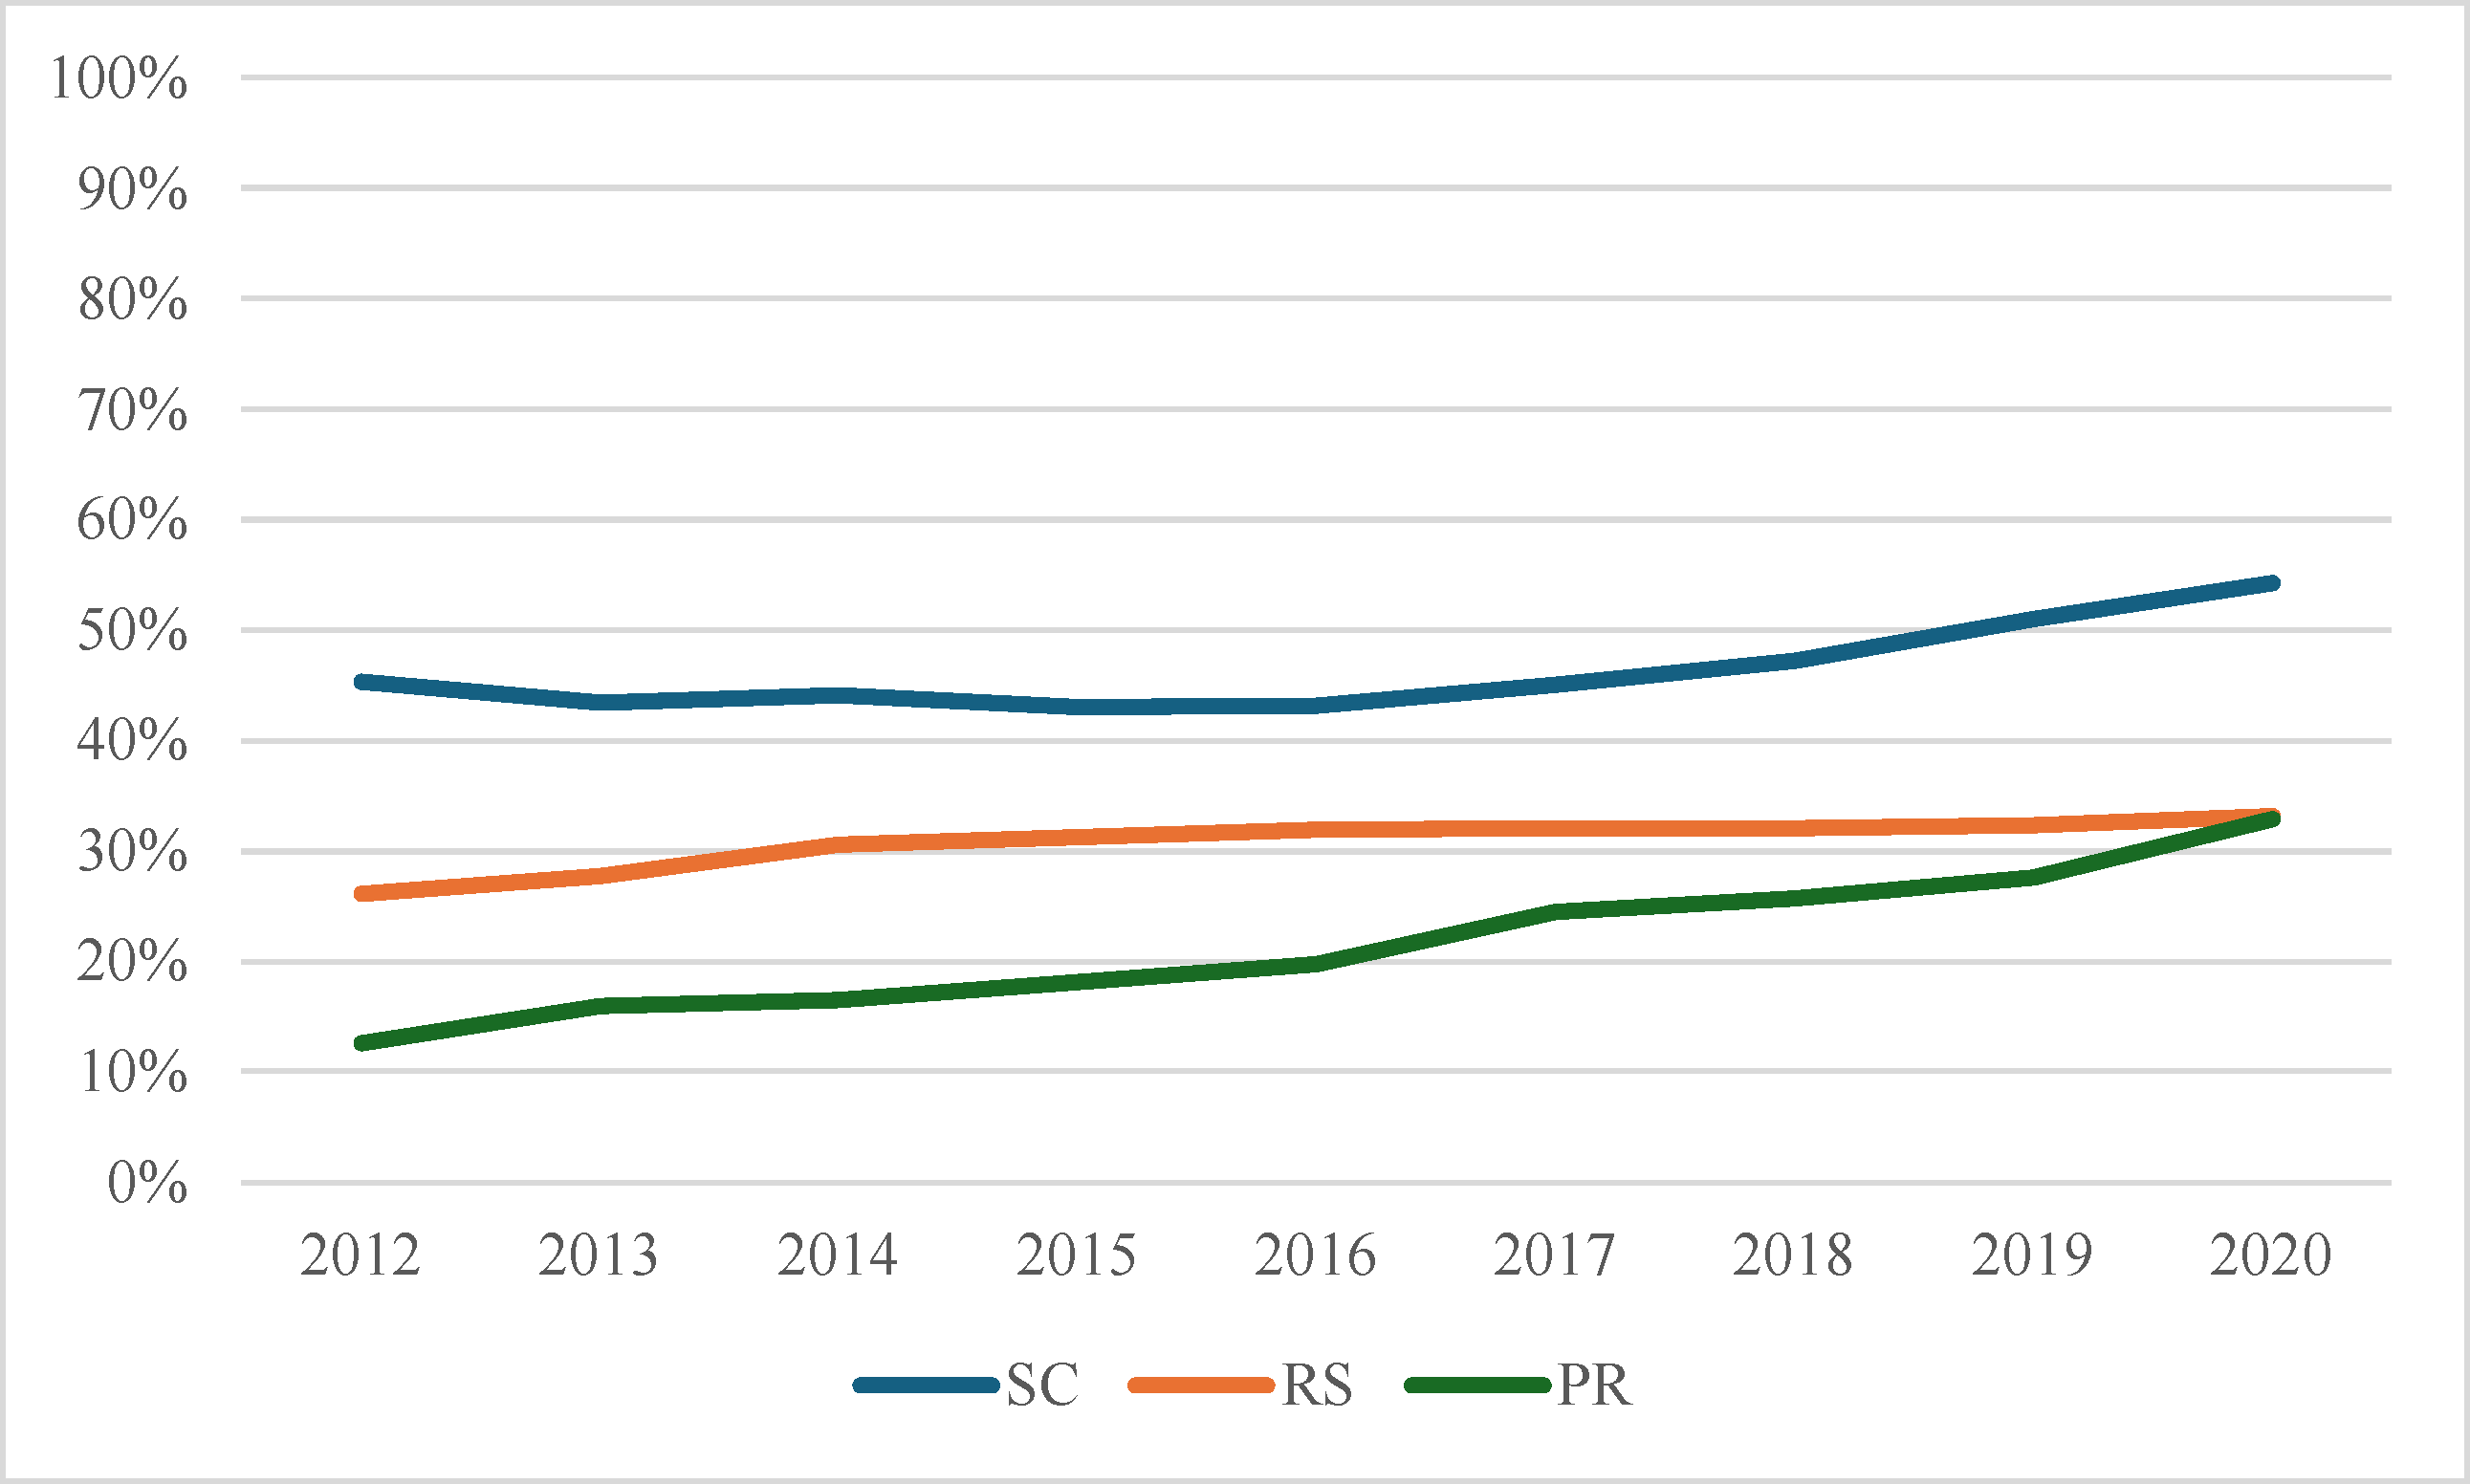
\includegraphics[width=5.0in]{imagens/faltantes-sul.pdf}
    \fonte{Datasus - Sinasc}
    \label{graf:sul}
\end{grafico}

\begin{grafico}
    \centering  
    \caption{Percentual de dados faltantes para a idade do pai ou responsável - Região Norte - 2012-2020}
           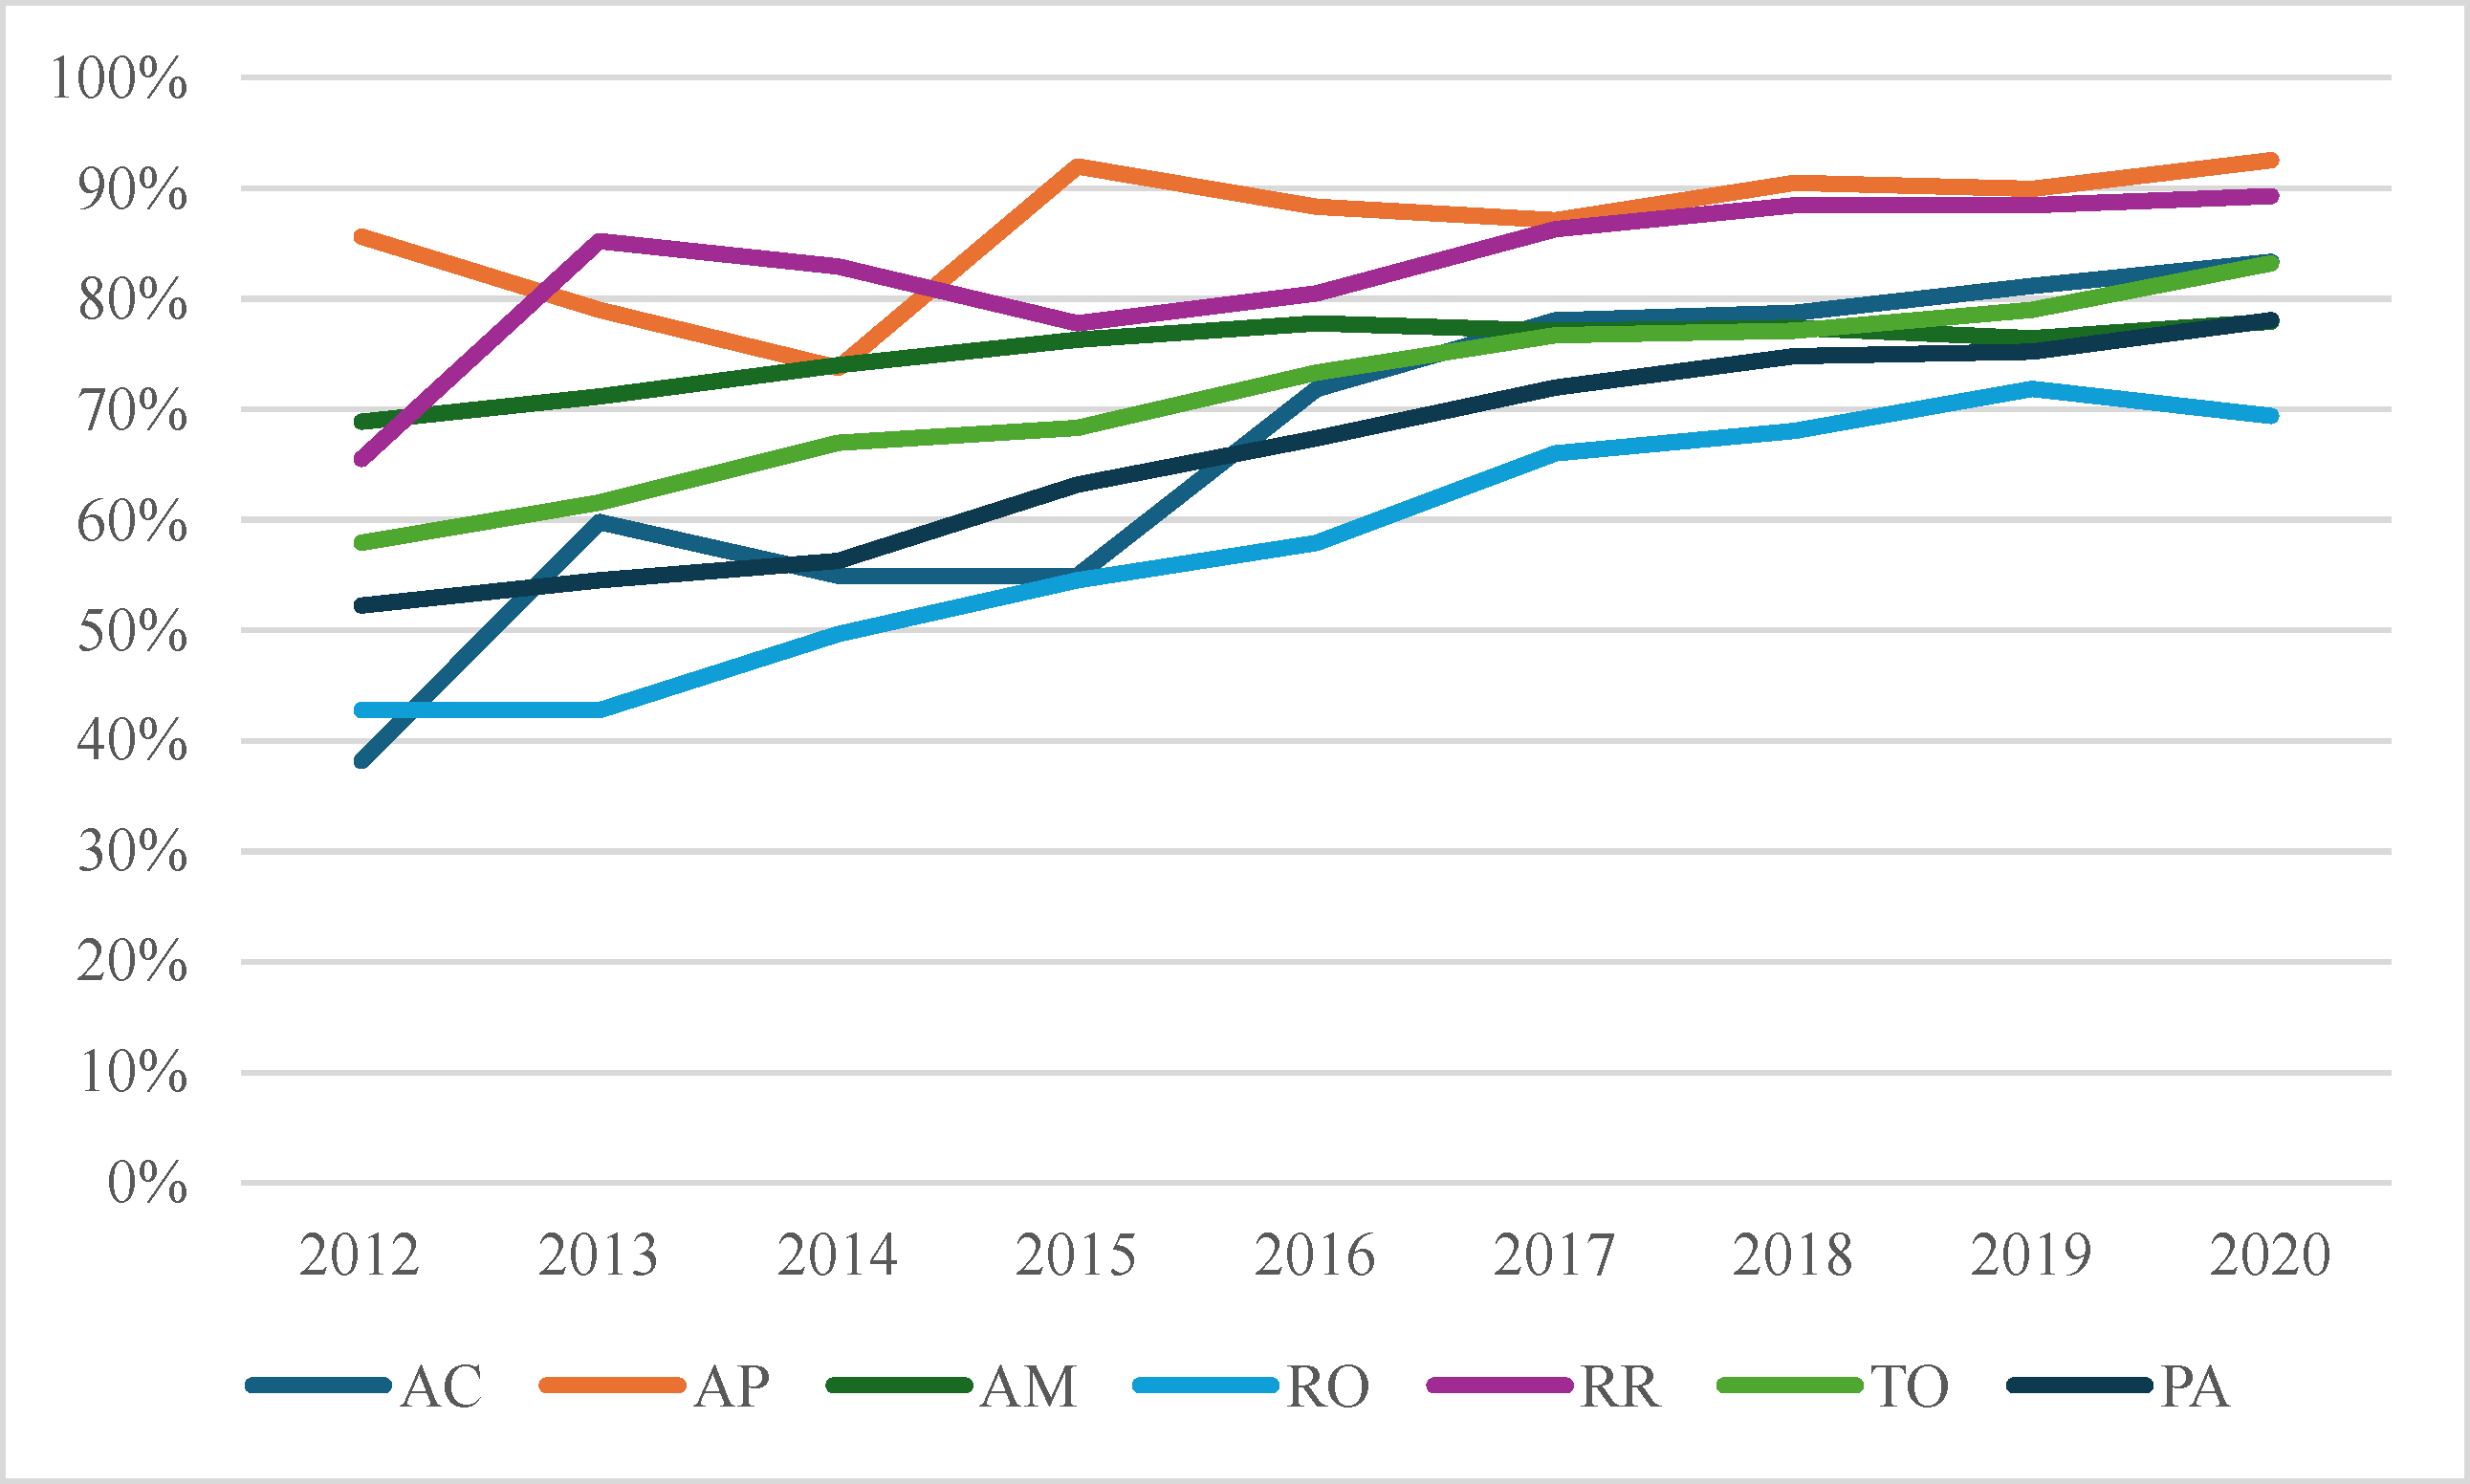
\includegraphics[width=5.0in]{imagens/faltantes-norte.pdf}
    \fonte{Datasus - Sinasc}
    \label{graf:norte}
\end{grafico}

\begin{grafico}
    \centering  
    \caption{Percentual de dados faltantes para a idade do pai ou responsável - Região Centro-Oeste - 2012-2020}
   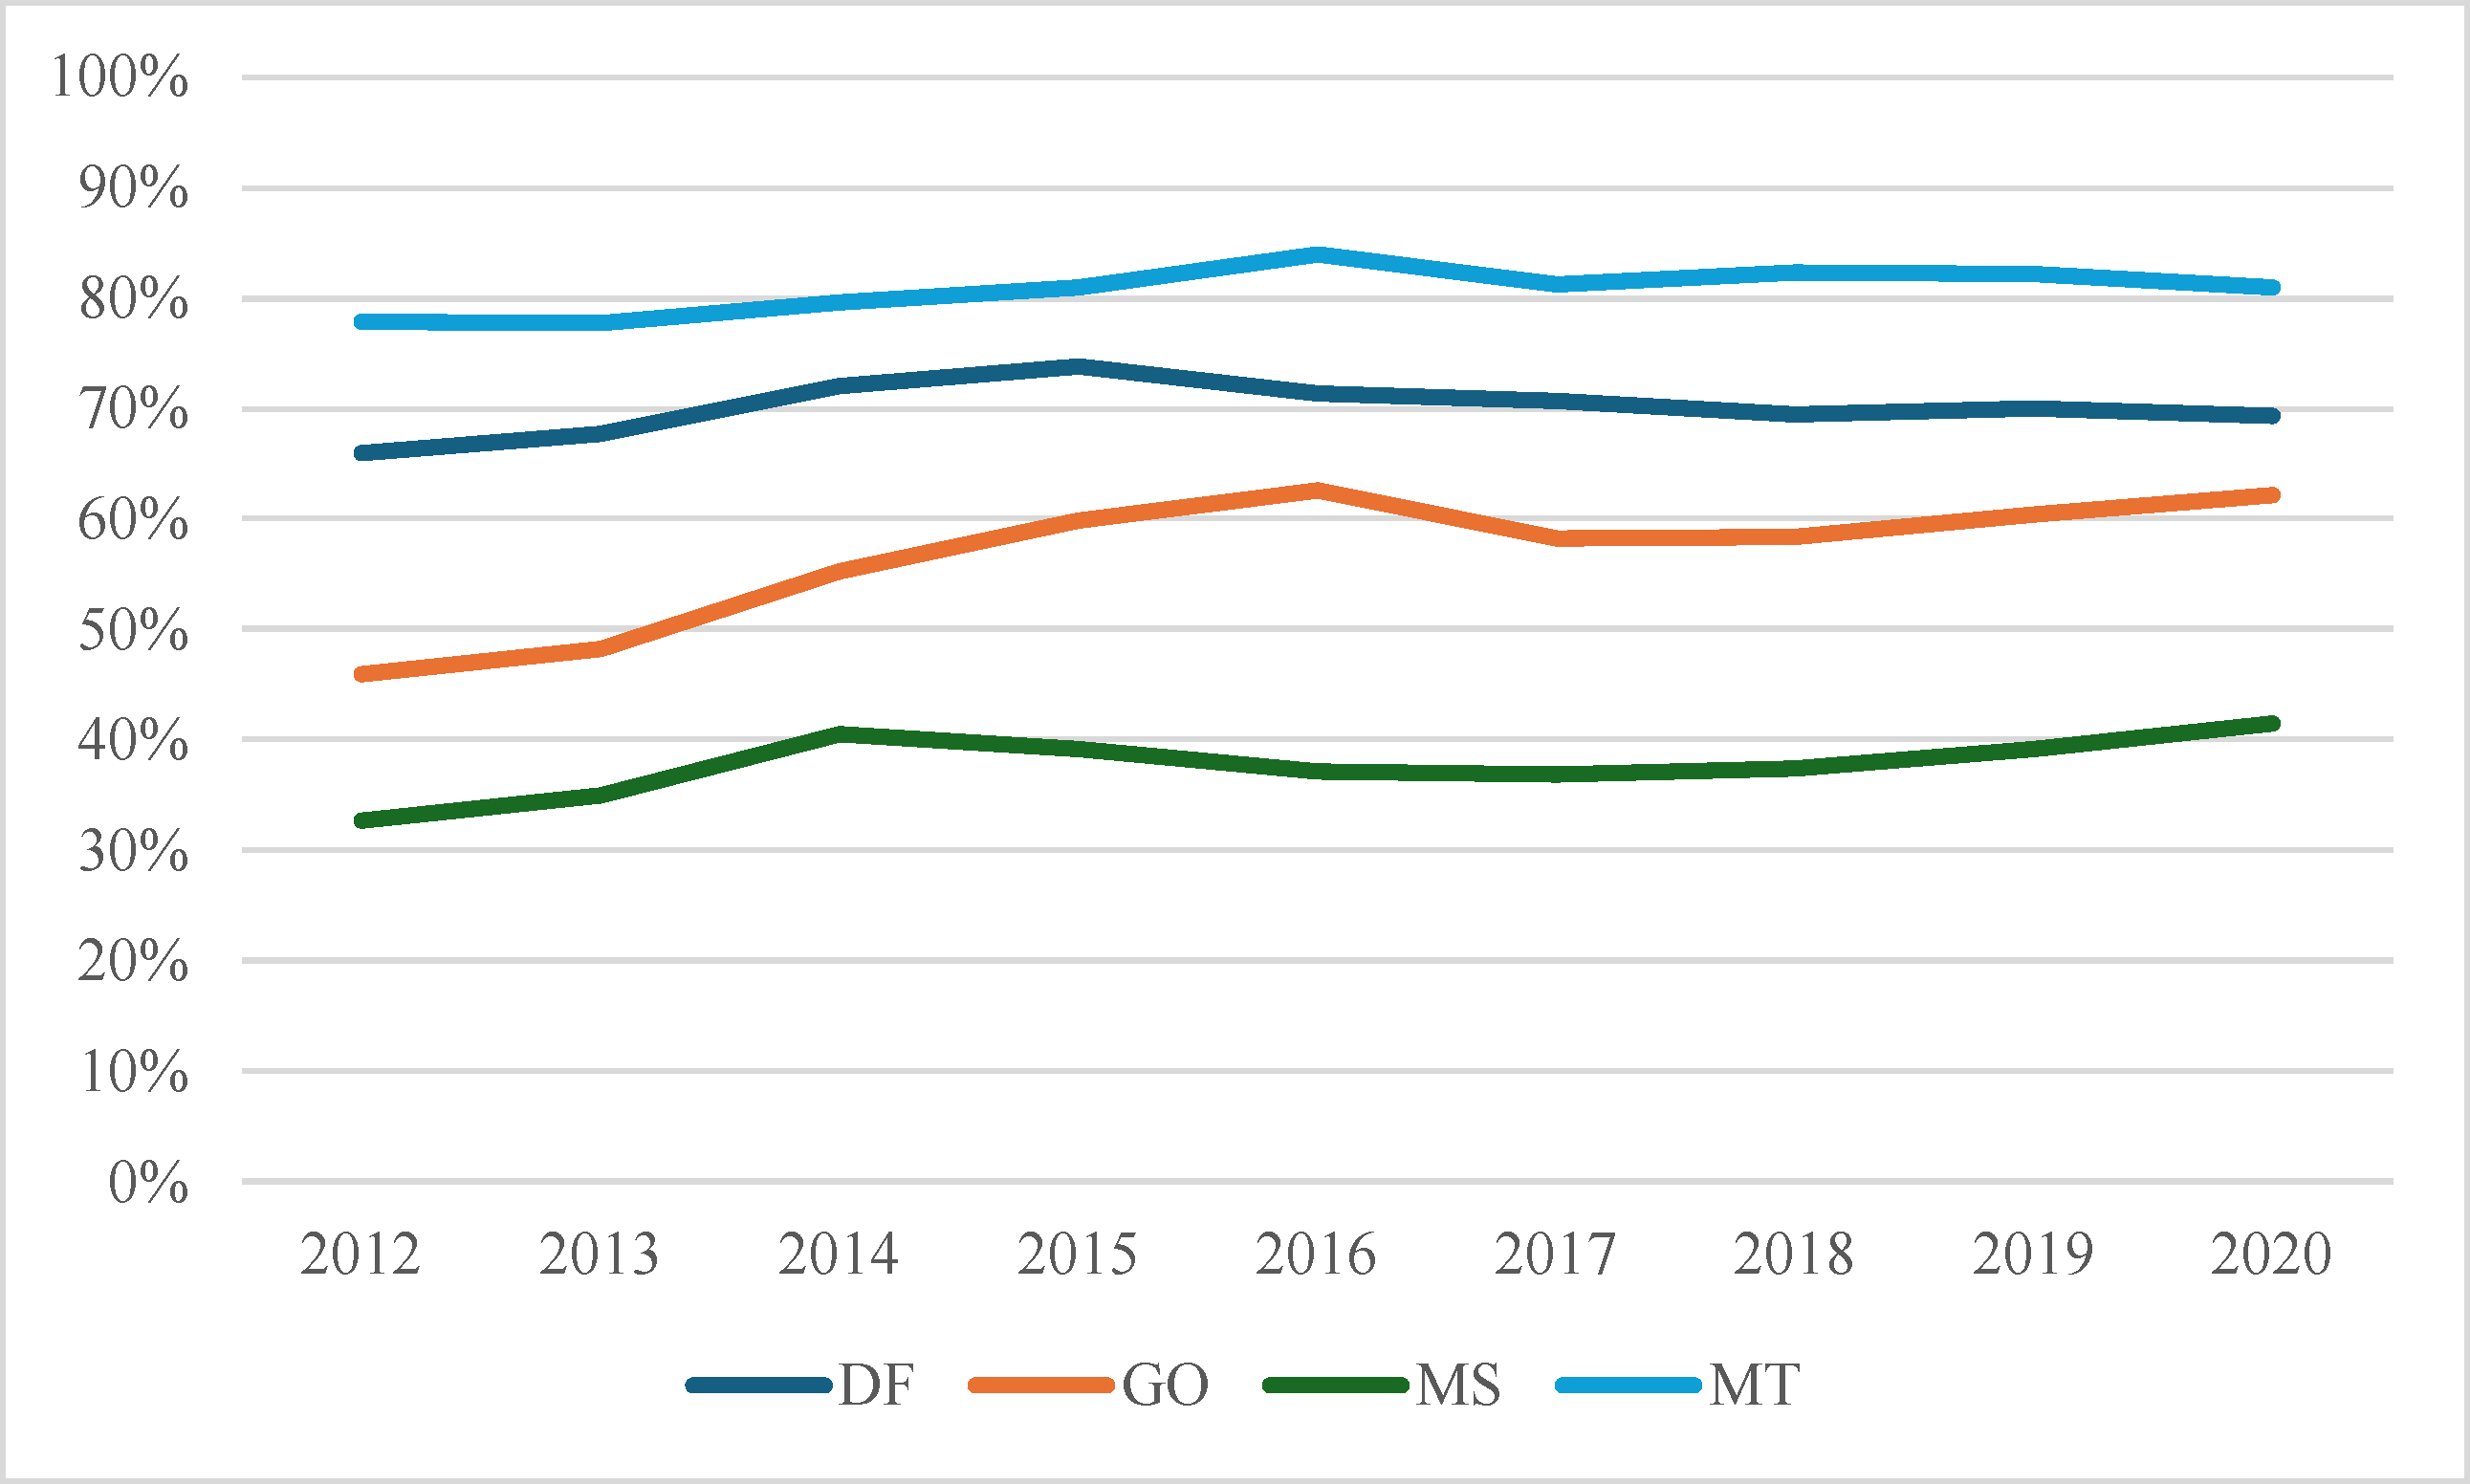
\includegraphics[width=5.0in]{imagens/faltantes-centro-oeste.pdf}
    \fonte{Datasus - Sinasc}
    \label{graf:centro-oeste}
\end{grafico}

\begin{grafico}
    \centering  
    \caption{Percentual de dados faltantes para a idade do pai ou responsável - Região Nordeste - 2012-2020}
        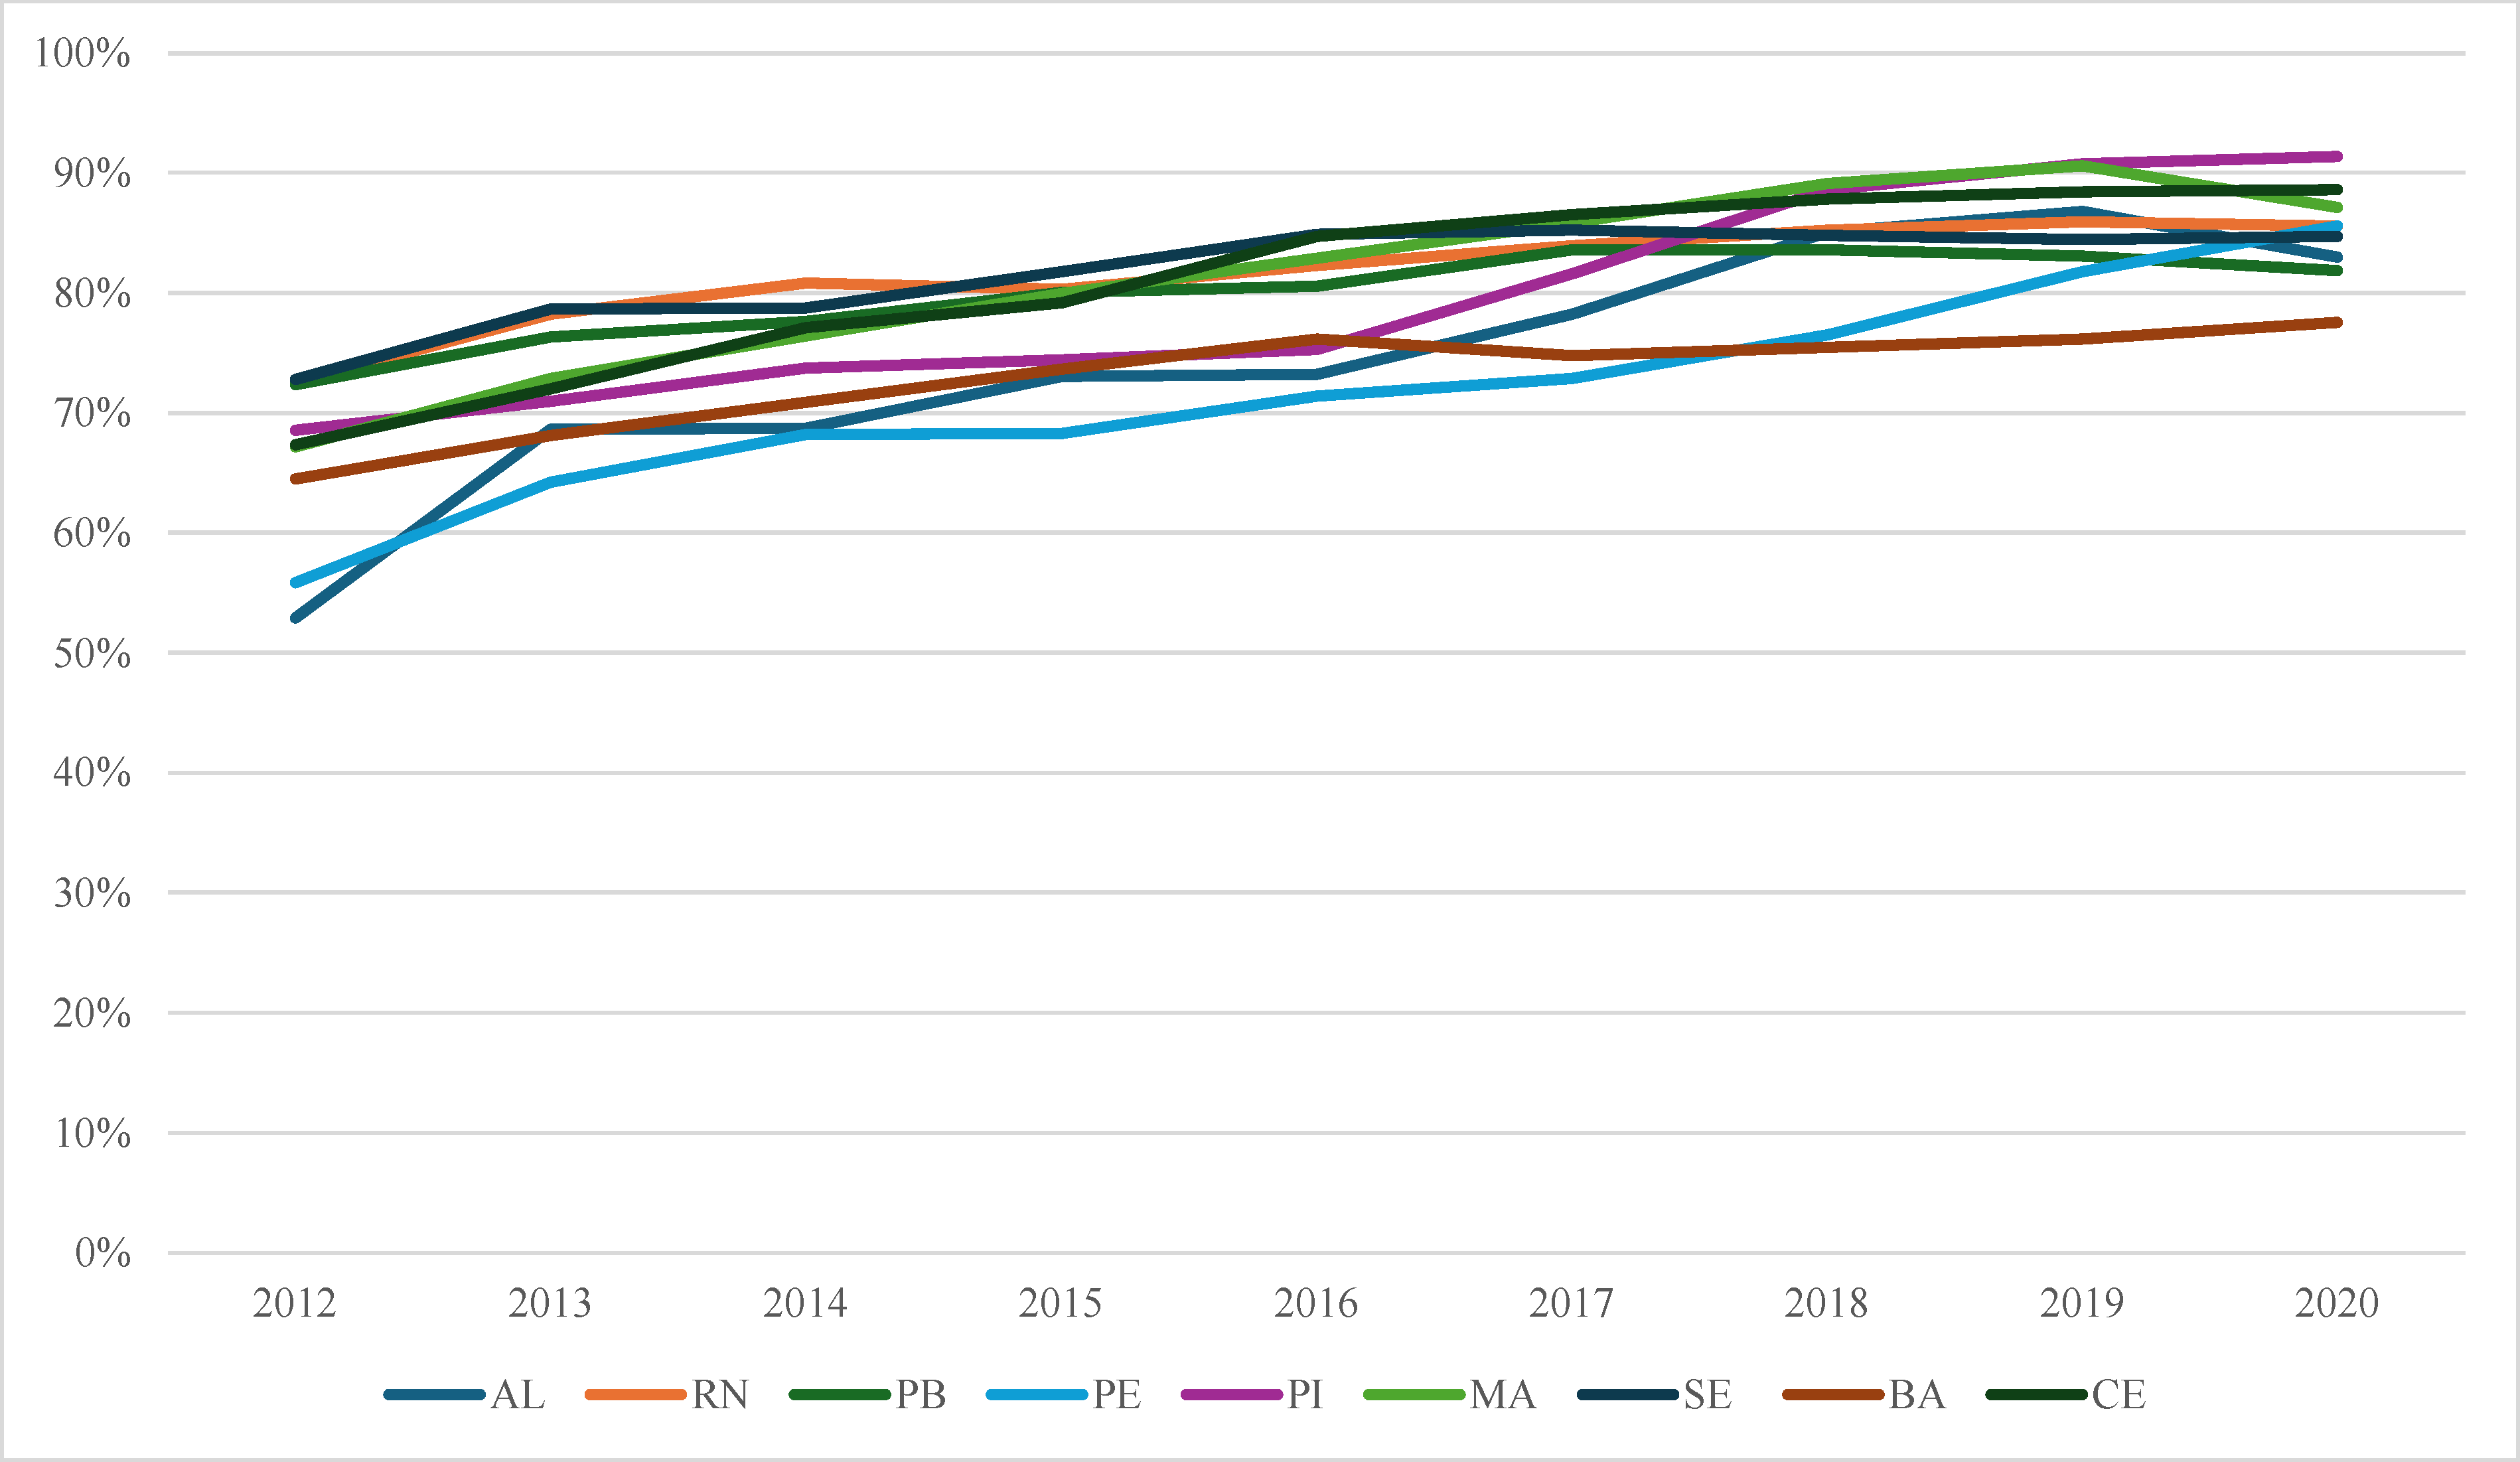
\includegraphics[width=5.0in]{imagens/faltantes-nordeste.pdf}
    \fonte{Datasus - Sinasc}
    \label{graf:nordeste}
\end{grafico}

Na região Norte (\ref{graf:norte}), a proporção de dados faltantes entre as UFs varia de forma menos suavizada através dos anos. Acre e Roraima, por exemplo, apresentam uma diferença de 22\% e 20\% (respectivamente) nos percentuais de dados faltantes de 2012 e 2013. O Amapá apresentou os piores níveis do país em 2012, 2015, 2016, 2017, 2018 e 2020. Em 2020, as UFs apresentaram 93\% de valores não observados, sendo esse o pior cenário entre as UFs no período entre 2012 e 2020.


Os dados da região Centro-Oeste demonstram certa estabilidade nos níveis diferentes de valores faltantes para as UFs. O Mato Grosso apresentou os piores níveis para todos os anos na região, mantendo uma diferença maior que 40\% até 2019 em relação ao Mato Grosso do Sul, a UF com melhores níveis da região. Em 2020 a diferença entre os estados alcança 39\%, a partir de uma suave melhora do Mato Grosso e uma leve piora do Mato Grosso do Sul.

O gráfico \ref{graf:nordeste} demonstra que o Nordeste, enquanto região, apresentou os maiores níveis de valores não observados. Nenhuma das UFs chega a alcançar um nível de pelo menos metade de preenchimento para a variável. Apresentam estabilidade em níveis altos para a proporção de valores faltantes para a idade do pai ou responsável. 





\begin{comment}

          AVALIAR AS RAZÕES PARA O CAMPO SER MARCADO COMO IGNORADO OU SER DEIXADO EM BRANCO ----
        
           FALANDO SOBRE A VARIÁVEL ESCOLARIDADE DA MÃE, MAS ACREDITO QUE O MESMO VALE PARA INFORMAÇÕES SOBRE O PAI: 
        
        A incompletude da escolaridade da mãe foi caracterizada quando o campo da variável no Sinasc apresentava-se em branco ou preenchido como “ignorado”. Todavia,
        
        O campo marcado como ignorado pode estar associado a diferentes fatores. Enquanto em “branco” pode ter relação com o não preenchimento do campo pelo profissional; “ignorado” pode ser pela indisponibilidade de tal informação.
        Nesse ponto de vista, algumas publicações referiram que uma das restrições para a melhor completude da variável foi a ausência das informações no prontuário hospitalar e, para o seu preenchimento, haveria necessidade de uma entrevista com a puérpera ou seu acompanhante, o que, muitas vezes, torna-se difícil por conta de ela não estar em condições de responder ou do seu acompanhante não
        ter conhecimento sobre sua escolaridade, sendo necessária a busca de outras fontes como o cartão da gestante \cite{silvestrin2018avaliaccao}
        %https://www.scielosp.org/pdf/csp/2018.v34n2/e00039217/pt 
\end{comment}



%
\input{cap2-base/tratamento-variável}
